\chapter{演化网络}

\section{Essentials}

\subsection{防范意识对随机网络上的疾病传播的影响}
\href{https://www.sciencedirect.com/science/article/pii/S002251931930459X}{防范意识对随机网络上的疾病传播的影响}。文章中说流行病\textit{期间}产生的防范意识不会对basic reproduction number产生影响。从其他人群中产生的防范意识会降低$R_0$. 防范意识可以显著减小流行病的规模,切断与病人的连边比降低感染率的效果要明显得多。流行病规模不会随着防范意识和感染率单调减小。局部和全局的防范意识是否对流行病规模产生影响取决于网络的类型和感染率。

\subsection{偏好与地理对流行病传播的影响}
\href{https://journals.aps.org/pre/abstract/10.1103/PhysRevE.76.056109}{偏好与地理对流行病传播的影响}:随机网络上的SIS模型,每个时刻,空间网络增加一个有$m$条边的结点。它与度为$k_{j}$,距离为$d_{ij}$的结点$j$连接的概率正比于$k^{A}_{j}/d^{B}_{ij}$, $A$和$B$都是正常数。如果$A=0$, 就是有临界值的普通疾病传播,疾病最终会消失;$B=0$时,(a) $A=1$时没有临界行为,其他时候仍然有临界行为。如果两个因素同时存在,临界值之上的~$A$和临界值之下的~$B$控制的网络对于传染是有鲁棒性的。

\subsection{Epidemic thresholds in dynamic contact networks}
\href{https://royalsocietypublishing.org/doi/pdf/10.1098/rsif.2008.0218}{Epidemic thresholds in dynamic contact networks}再生率$R_0$是流行病学中的基本量,它决定了易感群体中传染病的一阶增长。在大多数流行病的\textbf{理论模型}中,都有一个特定的值$R_0$,即流行病阈值,高于该值可能会大流行,但低于此值就不会发生大流行。随着流行病模型的复杂性增加,计算流行病阈值的难度也增加。本文通过简单的动态随机网络类推导了SIR流行病的$R_0$和流行阈值。与大多数流行病学模型一样,$R_0$取决于两个基本流行病参数,即传播率和恢复率。我们发现,$R_0$还取决于社会参数,即描述并发联系人数量异质性的\textbf{度分布}以及给出联系人启动和终止速率的混合参数。我们表明,社会融合从根本上改变了流行病学格局,因此,用静态网络来近似动态网络可能是不足够的。

几个简写:neighbour exchanges (NEs)

任意度分布的静态随机网络已经有很多研究在做了(Callaway et al. 2001; Newman et al. 2001, 2002; Chung \& Lu 2002; Catanzaro et al. 2005)。我们假设一个度分布为$\{p_k\}$的网络。对于大型的网络,给定一条ego到$x$边,$x=alter$的概率正比于alter的度。用 $\{ego, alter\}$来记录一条边; $(ego, alter)$ 来记录ego到alt的联系。

\section{随机图上疾病和信息的传播}

\href{https://www.pnas.org/content/pnas/107/10/4491.full.pdf}{Some features of the spread of epidemics and information on a random graph}. 

\paragraph{三种随机图}\textbf{小世界}图是Watts和Strogatz引入的。在一维圆环$\mathbf{Z} ~\text{mod}~n$上,连接所有距离小于等于$m$的点。然后以概率$p$,将边的一端连到纯随机的另一个结点上。\textbf{BA模型}依次加入结点,连接$m$条边到已有结点上,概率正比于该结点的度。该模型的度分布收敛于\begin{equation} p_{k}=\frac{2 m(m+1)}{k(k+1)(k+2)} \quad \text { for } k \geq m \end{equation}如果不是正比于度,而是一个平移项$k+a$ ($a>-1$), 那么度分布将会是$p_k\sim C k^{-3+a}$. 如果$a\geq 0$, 这种方式等价于:新边以概率为$a/(a+1)$随机选一个结点,以概率为$1/(a+1)$使用偏好依附机制。\textbf{NSW模型},给定度分布$\{p_k,k\geq 0\}$, 独立采样出真实的度序列$\{d_k\}_{k=1,\dots, n}$, 假设采样出的度的和为偶数,然后结点依次随机连$d_i$条边,构建一个$n$个结点的随机图$G_{n}$. 

\paragraph{两种流行病}\textbf{SIR}类似于分枝过程,以速率为$\lambda$感染,以速率为$1$恢复,恢复之后不易感。该模型与渗流模型有很好的对应。如果$x$, $y$在图里是邻居,就以概率为$\lambda/(\lambda+1)$, 也就是二者之一患病期间感染另一人的概率,连边。流行病的规模就是含有初始被感染结点的连通图的大小。\textbf{SIS}模型要更复杂一些。感染和恢复速率分别是$\lambda$和$1$. 这又称为\textit{接触过程}。

\textbf{小世界网络}的简单版本$m=1$在Watts和Strogatz的小世界十年前就被Bollobas和Chung提出了。这种小世界的半径是$\sim\log_2 n$. 称为BC小世界。我们希望每个个体有且只有一个长程联系,这样就可以定一个相关的大世界图$\mathscr{B}_m$. 

自由积是个不错的形式。$\mathbf{Z}*\{0,1\}$. 其中的元素的形式是$z_01z_11\dots 1z_k$. 也就是移动$z_0$连到$1$, 然后到$z_{1}$再到$1$以此类推。这个文章太难了我以后再看吧。不过真的好精彩。

\href{https://journals.aps.org/pre/pdf/10.1103/PhysRevE.82.036112}{演化网络上的疾病传播}

\subsection{适定性网络上的流行病动态}
\href{https://journals.aps.org/prl/abstract/10.1103/PhysRevLett.96.208701}{Epidemic Dynamics on an Adaptive Network}

易感者能够通过重新连接其网络连接来避免与感染者接触。引起、分类度相关性,振荡,磁滞和一阶跃迁。

考虑例如在社交网络上传染病的传播。人类倾向于通过\textbf{避免与感染者接触}来应对这种流行病。局部连接的这种重新布线可对疾病的动力学产生强烈影响,进而影响重新布线过程。因此,出现了时变网络拓扑与节点动态之间的复杂交互。自适应网络上的SIS模型可以证明,用于网络连接的简单直观的重连规则对网络具有深远的影响,并且能够生成特定的网络属性,例如广度分布,分类度相关性以及两个松散连接的子隔间的形成。\textbf{动力学上的结果}是出现了新的流行阈值(对应于一阶跃迁),多个稳定平衡的共存(导致磁滞)以及振荡机制的出现,所有这些在静态SIS网络中都是不存在的。

考虑结点数为 $N$, 边数为 $K$ 的网络上的SIS过程。每个时间节点上,每个S-I边以概率 $p$ 变成I-I;每个I以概率为 $r$  恢复健康。\textbf{重连}体现在:S可以通过重连来保护自己。SI以概率为 $w$ 被打断,连接到一个随机的健康S结点。

\paragraph{流行条件}考虑临界感染概率$p^*$. 在不重连的网络上,基本再生数$R_{0}:=p\langle k\rangle / r$, 其中 $\langle k\rangle=2 K / N$,它表示由其他易受感染的网络上的单个感染节点引起的继发感染数。所以,给定网络结构,需要一个二级感染的话,$p^* = t/\langle k \rangle$. 如果考虑网络重连的话,一个 I 结点平均每次会失去 $w$ 比例的邻居。邻居数将是 $k(t)=\langle k\rangle \exp (-w t)$. 由于 I 的周期时$1/r$, 阈值将是\begin{equation}
    p^{*}=\frac{w}{\langle k\rangle[1-\exp (-w / r)]}\label{eq:rewire_threshold}
\end{equation}
由于$w\gg r$时,$p^* = w/\langle k\rangle$, 所以高重连率会使得流行病阈值提高很多,进而减小流行病的程度。

分几种情况:

\paragraph{重连与状态独立}

度分布是泊松分布,给定结点二阶邻居的平均度 $\langle k_{nn} \rangle$ 与度 $k$ 是独立的。

\paragraph{上面的重连规则}

先让SIS机制关掉,即 $r = p = 0$. 设 I 的比例是 $i$, $S$ 的比例是 $s = 1-i$, 都是常数。但是 SI 边随时间不断减少,逐渐变成不在一起的两个组团。假设我们从一个随机图开始,各种类型边的密度分别是 $l_{SS}=s^2\langle k\rangle /2 $, $l_{II}=i^2\langle k\rangle /2 $, $l_{SI}= \langle k\rangle /2 - l_{II} - l_{SS} = si\langle k\rangle $. 有适定性重连规则之后,稳定状态下所有的 SI 边都会转为 SS 边,密度是 $l_{SS} = (1-i^2)\langle k \rangle/2$. 因此,S 与 I 在不同的度分布 $\rho_k$ 假定下,S 的平均度 $\langle k_S \rangle = (1+i)\langle k\rangle $, I 的平均度 $\langle k_I \rangle = i\langle k_I \rangle$. 虽然各自还是泊松的,但是 S 组团的联通度更高。由于 $ \langle k_{nn} \rangle$ 与两个集团中分别的度 $k$ 都是独立的,组团内部的度关联也消失了。但是如果两个组团考虑在一起,一个\textit{净度关联} $r_\text{corr} > 0$ 可以出现,因为 $\langle k_{nn} \rangle$ 对于 S 组团更大。

\begin{figure}
    \centering
    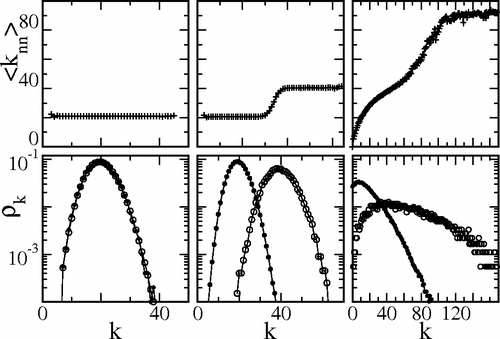
\includegraphics[width = 0.5\linewidth]{Pics/rewire-structure-of-adaptive-networks.png}
    \caption{适定性网络的结构。上边一行是平均最近邻度$\langle k_{nn} \rangle$, 下面一行是度分布。从左到右分别是无差别重连/没有SIS关系的/适定性网络。参数设置是$w = 0.3$, $r = 0.002$, $p = 0.008$, $N = 10^5$, $K = 10^6$.}\label{fig:rewire-structure}
\end{figure}

最后,同时考虑适定性重连与流行病动力。虽然重连没有快到可以完全分离 S 与 I,但是还是能形成两个比较松散连接的组团,比如说 $l_{SI} \approx 0.01\langle k \rangle$. 组团间联系在被切断,有的 I 结点也在康复,有的 S 结点也在被感染。这导致结点度随时间的巨大变化。只要一个结点是 S,它的度几乎就以线性增长,\begin{equation}
    \dot{k} = wl_{SI}.
\end{equation} 反之,感染的结点的度以指数递减,\begin{equation}
    \dot{k} \sim -wk.
\end{equation}所以存在一个复杂的均衡,组团间和组团内的边,S 与 I 的密度都是一个常数。这个均衡中,连续的重连会维护一组 S 与 I 的度分布,以及一个正的度关联(高高相连,低低相连)。

\paragraph{进一步的性质}
\begin{figure}
    \centering
    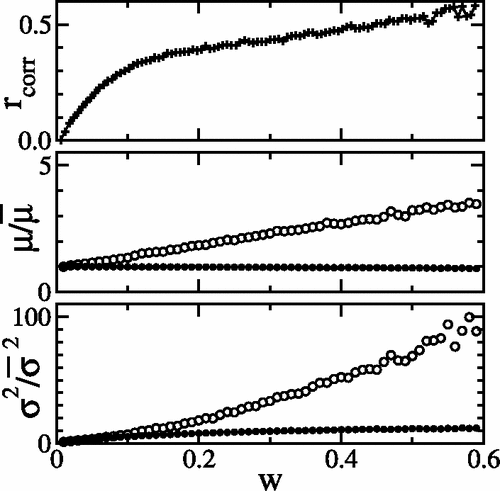
\includegraphics[width = 0.5\linewidth]{Pics/Degree_correlation_index.png}
    \caption{上图是$r_\text{corr}$作为$w$的函数,下图是度分布的均值和方差作为$w$的函数。空心是 S,实心是 I. 都相对于没重连的情况标准化了。参数是$N=10^5$, $K = 10^6$, $r = 0.002$, $p = 0.008$.}\label{fig:parameters_vs_rewire}
\end{figure}

图~\ref{fig:parameters_vs_rewire}~进一步量化了自适应重新布线对新兴网络结构的影响。随着$w$的增加,相关度迅速增加。此外,易感者的平均程度增加而感染程度则略有下降。甚至更明显是在易感的度分布的方差的增加。比如$w=0.6$时的方差$\sigma^2$大了100倍。这表明形成了牢固连接的中心和临时孤立的节点,这些节点由重连而迅速重新连接。

适应性重连促进了受感染个体的隔离,这可以大大提高流行阈值。然而,这样做时,连引入了人口中连接的混合,并且还导致形成高度连接的易感簇,其特征在于度分布的方差较大,因此具有较低的流行阈值。因此,重连的局部作用趋于抑制流行,而产生的拓扑作用则促进流行。所以重连有两个相反的作用。

为了研究这个问题,我们考虑一个低维问题中的 $l_{SS}$ 和 $l_{II}$. 利用moment closure approximation方法。对于$a,b,c\in[S,I]$做如下近似:$l_{abc} = l_{ab} l_{bc} / b$. 这样的系统上面就有如下的ODE:
\begin{align}
    \frac{d}{d t} i&=p l_{\mathrm{SI}}-r i\\
    \frac{d}{d t} l_{\mathrm{II}}&=p l_{\mathrm{SI}}\left(\frac{l_{\mathrm{SI}}}{s}+1\right)-2 r l_{\mathrm{II}}\\
    \frac{d}{d t} l_{\mathrm{SS}}&=(r+w) l_{\mathrm{SI}}-\frac{2 p l_{\mathrm{SI}} l_{\mathrm{SS}}}{s}
\end{align}
它可以与数值模拟的结果,也就是图~\ref{fig:bifurcation_diagram}。在不重新布线的情况下,只有一个连续的动态过渡发生在流行阈值$p^∗$上。随着重连,该阈值与等式~\ref{eq:rewire_threshold}完全吻合。但同时,也会出现\textbf{一个较低的鞍点分叉}。该点之上,已有的流行病会继续存在。与没有重连相比,两个流行病机制之间出现了不连续一阶相变(导数就不连续了)。其之间有双稳定状态,健康和流行病可能都是稳定的。所以,会形成一个\href{https://baike.baidu.com/item/滞后回线/360581?fr=aladdin}{滞后曲线}。

\begin{figure}
    \centering
    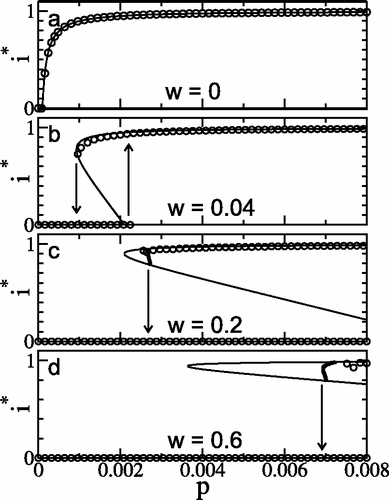
\includegraphics[width = 0.5\linewidth]{Pics/bifurcation_diagram.png}
    \caption{I 的密度作为传染概率$p^*$的函数,对于不同的重连概率$w$.}
    \label{fig:bifurcation_diagram}
\end{figure}

数值模拟表明,滞后回线和一阶跃迁的存在是自适应模型的通用特征,可以在所有有限的重连速率下观察到。虽然增加重连速率几乎不会减少局部流行病的规模,但滞后的阈值的性质会在更高的重连速率下发生变化。首先,亚临界Hopf分支产生了不稳定的极限循环,从而取代了鞍点分支。在更高的重连速率下,Hopf分支变得超临界。 由于现在出现的极限周期是稳定的,因此Hopf分叉标志着第三阈值,在该阈值处会发生连续向振荡动力学的过渡。但是,这些振荡只能在遇到持久性阈值之前在相对较小的参数区域(请参见图~\ref{fig:2-para-phase})中观察到,该阈值现在对应于循环的折叠分叉。

\begin{figure}
    \centering
    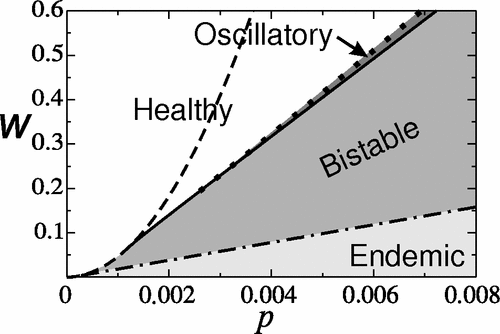
\includegraphics[width = 0.5\linewidth]{Pics/2-para-bifurcation.png}
    \caption{两个参数的相图。}
    \label{fig:2-para-phase}
\end{figure}

\section{本章Ideas}

\subsection{戴口罩的演化博弈}

\section*{演化机制}